%
% Layout retirado de http://www.di.uminho.pt/~prh/curplc09.html#notas
%
\documentclass{report}
\usepackage[portuges]{babel}
\usepackage[utf8]{inputenc}
\usepackage[latin1]{inputenc}
\usepackage{graphicx}
\usepackage{tipa}
\usepackage{parallel,enumitem}

\usepackage{url}
\usepackage{enumerate}

%\usepackage{alltt}
%\usepackage{fancyvrb}
\usepackage{listings}
%LISTING - GENERAL
\lstset{basicstyle=\small,
    numbers=left,
    numberstyle=\tiny,
    numbersep=5pt,
    breaklines=true,
    frame=tB,
    mathescape=true,
    escapeinside={(*@}{@*)}
}

\usepackage{xspace}

\parindent=0pt
\parskip=2pt

\setlength{\oddsidemargin}{-1cm}
\setlength{\textwidth}{18cm}
\setlength{\headsep}{-1cm}
\setlength{\textheight}{23cm}

\def\darius{\textsf{Darius}\xspace}
\def\antlr{\texttt{AnTLR}\xspace}
\def\pe{\emph{Publicação Eletrónica}\xspace}

\def\titulo#1{\section{#1}}
\def\supers#1{{\em Supervisores: #1}\\ }
\def\area#1{{\em \'{A}rea: #1}\\[0.2cm]}
\def\resumo{\underline{Resumo}:\\ }


%%%%\input{LPgeneralDefintions}

\title{Projeto (3º ano de LCC)\\ \textbf{VMS, um Simular Visual para a Máquina de Stack Virtual VM}\\ Relatório de Desenvolvimento}
\author{Adriano Campinho\\ (a79032) \and Vasco Leitão\\ (a79220) }
\date{\today}

\begin{document}

\maketitle
\begin{abstract}
	\quad Este documento apresenta o relatório desenvolvido no âmbito da Unidade Curricular de Projecto, do curso de
	Licenciatura em Ciências da Computação, Universidade do Minho, no segundo semestre do ano letivo 2017/2018.\\
	\quad Pretendendo-se explicitar o processo de conceção e implementação do mesmo, assim como as escolhas tomadas e as pretendidas resoluções
	para cada problema exposto no enunciado fornecido, prestando especial atenção ao modo de utilização do simulador; \\
	\\
	\\
	\\
    \\
	\supers{Pedro Rangel Henriques e José João}
	\area{Processamento de Linguagens}

\end{abstract}

\tableofcontents

\chapter{Introdução} \label{intro}

\quad Nos últimos anos, temos usado nas disciplinas de Processamento de Linguagens (e
Compiladores) a máquina virtual VM, uma máquina de stack que suporta inteiros, reais e
strings e tem uma heap para permitir um uso dinâmico da memória (necessário por exemplo
para implementar listas ligadas). A VM é programada em Assembly e que disponibiliza um
conjunto de instruções máquina mínimo e muito compreensível, o que a torna
pedagogicamente muito relevante como máquina objeto (destino) em tarefas de compilação.
\\
\\
\null\quad Para que o uso da VM seja realmente um bom instrumento de trabalho nestes cursos, é
fundamental que exista um simulador que permita testar (de preferência passo a passo) o
código gerado. Atualmente existe, como é de conhecimento de todos, um Assembler para
traduzir o Assembly produzido numa lista de códigos máquina e existe um interpretado que
executa esse código e que fornece uma interface visual que permite acompanhar a execução
verificando a evolução dos vários blocos de memória e dos registo de controlo da máquina.
\\
\\
\null\quad Esta versão, codificada em Java, está funcional e pode ser usada, mas tem alguns problemas de
implementação, nomeadamente o elevado tempo de execução, quando os programas
aumentam um pouco.
\\
\\
\null\quad Neste projeto pretende-se que os alunos reconstruam o simulador com interface interativo e
visual para a máquina VM desde o início, em Java ou em C (conforme preferência do grupo)
produzindo um executável que evite os problemas atuais.

\chapter{Análise e Especificação} \label{ae}
\section{Descrição Informal da Máquina}

\quad Trata-se duma máquina de pilhas (por oposição às máquinas de registos). Esta é composta duma pilha de execução, duma pilha de chamadas,
duma zona de código e de duas heaps:

\begin{center}
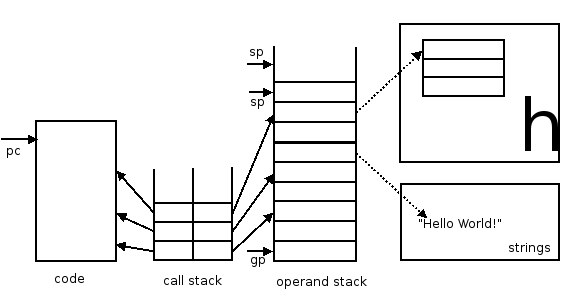
\includegraphics{stacks.png} \\
\caption { Diagrama organização maquina VM }
\end{center}

\paragraph{\quad Code Block -}
Esta pilha contém o conjunto das instruções do programa. Esta é preenchida no inicio da execução do programa, mantendo-se igual
do princípio ao fim da execução do mesmo;
\paragraph{\quad Operand Stack -}
Esta pilha contém valores guardados no registo da maquina. Estes são todos indexados, podendo ser do tipo inteiro, real e endereço;
\paragraph{\quad Heap Stack -}
Esta pilha contém cadeias de caracteres (strings), cada uma destas referenciado por endereços, cada bloco,
contendo um certo numero de caracteres;
\paragraph{\quad Call Stack -}
Esta pilha contém blocos estruturados, cada um destes referenciado por endereços, cada bloco
estruturado contém um certo numero de valores (estes são do mesmo tipo dos que se podem encontrar na Operand Stack);
\\
\\
\null\quad Um endereço pode apontar para quatro tipos de informação: para código, para a
pilha, para um bloco estruturado ou para uma string.
Ao longo da execução do programa são guardados os seguintes quatro registos:
\begin{itemize}
	\item \textit{\textbf{SP}} (Stack Pointer) o registo aponta para o topo corrente da pilha/ para a primeira célula livre da pilha.
	\item \textit{\textbf{FP}} (Frame Pointer) o registo aponta para o endereço de base das variáveis locais.
	\item \textit{\textbf{GP}} (Global Pointer) o registo contém o endereço de base das variáveis globais.
	\item \textit{\textbf{PC}} (Program Counter) o registo aponta para a instrução corrente (da zona de código) por executar.
\end{itemize}

A pilha de chamada permite guardar as chamadas: contém pares de apontadores
(i, f). O endereço i guarda o registo de instrução pc e f o registo fp.

\subsubsection{Instruções}

\quad As instruções são designadas por um nome e podem aceitar um ou dois parâmetros.
Estes parâmetros podem ser dos seguintes tipos:
\begin{itemize}
\item Constantes inteiras,
\item Constantes reais,
\item Cadeias de caracteres delimitadas por aspas. Estas cadeias de caracteres seguem as
mesmas regras de formatação que as cadeias da linguagem C (em particular no que
diz respeito aos caracteres especiais como \", \n ou \textbackslash\textbackslash ),
\item Uma etiqueta simbólica designando uma zona no código.
\end{itemize}

\quad O conjunto das instruções pode ser encontrado no documento original fornecido com as fontes da maquina virtual aqui descrita.
Destas foram ignoradas as primitivas gráficas, não sendo esta uma implementação de uma versão gráfica da maquina virtual;

\section{Planeamento e objetivos}
\quad O simulador deve ser implementado de forma a funcionar num maior numero de ambientes possível:
deve ser possível correr a simulação de vários modos possibilitando uma simulação interativa de cada programa.
Existindo a possibilidade do jogador interagir com a simulação através da linha de comandos ou através de uma Interface
gráfica a ser desenvolvida.\\
\null\quad Podemos então dividir o projecto em 3 grandes grupos:
\begin{itemize}
	\item \textbf{Parser:} O parser é responsável por percorrer o input do sistema e devolve
	os tokens, que correspondem a qualquer instrução, isto é, qualquer conjunto de símbolos que não incluam
	espaçamentos e mudanças de linha.
	\quad Por fim, o parser filtra também o texto por forma a remover qualquer ocorrência de espaçamentos e mudanças de linhas.
	Assim, o parser é responsável por processar o input para que este fique num estado que possa ser digerido pelo simulador,
	permitindo assim estabelecer uma maior diversidade de formatos de input que, mesmo não sendo totalmente aceites
	pelo processador, são mais completos e possuem uma componente estética maior.


	\item \textbf{Simulador:} um programa que através do input recebido do parser e, se necessário, do input do utilizador,
	faça a simulação em si do programa, permitindo que o utilizador controle a sua execução;

	\item \textbf{Interface Gráfica:} uma interface que permita ao utilizador interagir com a execução do simulador,
  dando-lhe acesso a informação sobre o estado atual da maquina;
	Cada vez que o utilizador interatue com a interface (e.g.\ clicando num botão), esta deve ser atualizada,
	refletindo as alterações feitas no estado na maquina e na interface.
\end{itemize}

\section{Especificação do Requisitos}
\quad Esta secção apresenta de forma mais especifica os requisitos de cada um dos grupos de desenvolvimento demonstrando os problemas que
surgiram durante cada fase:

\subsection{Parser}

\quad O parser deve aceitar programas com a seguinte sintaxe:

\begin{center}
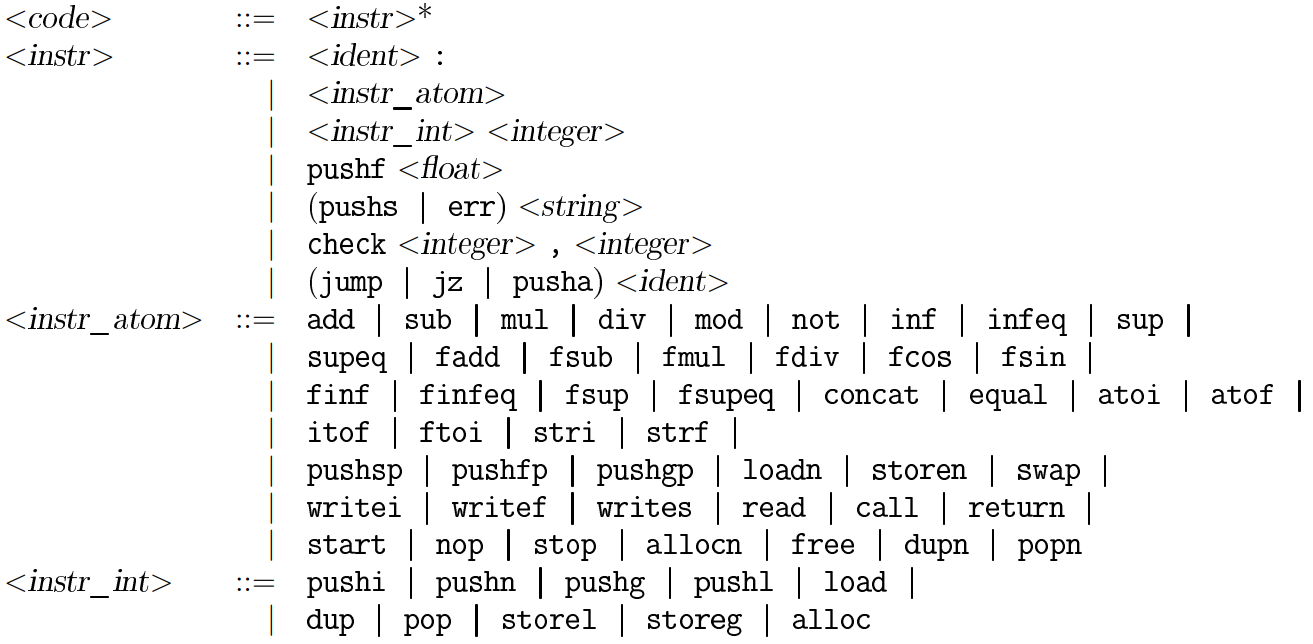
\includegraphics[width=\textwidth]{sintaxe.png}
\end{center}

%\subsubsection{Convenções lexicais:}

%\null\quad \textbf{\textless digit\textgreater} ::= [0-9]\\
%\null\quad \textbf{\textless alpha\textgreater} ::= [a-zA-Z]\\
%\null\quad \textbf{\textless label\textgreater} ::= [A-Z][A-Z0-9]*

%\null\quad \textbf{\textless comentario\textgreater} ::= \#.* \textvertline \space //\textspace\space.*

%\null\quad \textbf{\textless integer\textgreater} ::= -? \textless digit\textgreater + \\
%\null\quad \textbf{\textless float\textgreater} ::= -? \textless digit\textgreater + (.\textless digit\textgreater *?)\\

\quad Ainda, o parser deverá ignorar tudo o que sirva para embelezar o código do programa (sejam múltiplos espaços seguidos, linhas em branco ou mesmo
comentários por parte do criador do programa).

\subsection{Processador}

\quad O processador deverá receber o programa tratado pelo Parser e executar as instruções produzindo o resultado
esperado (descrito no documento referido acima), permitindo ao utilizador controlar a execução do programa;

\subsection{Interface Gráfica}
\quad A interface deve permitir ao utilizador executar as seguintes ações:
\begin{itemize}
\item Realizar 1 passo na execução do programa;
\item Realizar n passos (passado como argumento) na execução do programa;
\item Realizar a execução do programa ate ao fim de uma vez só;
\item Carregar um programa para ser simulado;
\item Recarregar o programa que esta atualmente a ser simulado;
\item Em qualquer momento da execução do programa, mostrar o estado actual da maquina (stacks e pointers);
\item Permitir ao utilizador introduzir input para o programa quando necessário;
\item Permitir ao utilizador introduzir múltiplas linhas de input de uma vez;
\item Carregar um ficheiro com o input para ser lido por um programa;
\end{itemize}

\chapter{Concepção/desenho da Resolução}
\section{Organização do código}

Em termos de organização do código, este foi dividido nos seguintes ficheiros:

\begin{itemize}
\item \textbf{README} - Este ficheiro contém uma lista de packages que necessitam de ser instalados para o correto funcionamento do simulador;
\item \textbf{structs/} - Pasta que contém os módulos das estruturas de dados criadas;
\item \textbf{vmsMan.1} - Este ficheiro é relativo a man page do simulador. Esta é acessível após a instalação da vms;
\item \textbf{lex.l} - Ficheiro lex referente ao parser, que contém todas as instruções e convenções necessárias;
\item \textbf{semantic.c} - A este ficheiro estão associadas as funçoes que dão significado as instruções, isto é, manipula as estruturas de acordo com a instrução;
\item \textbf{syntax.y} - Este ficheiro é processado pelo yacc e gera o código c que trata de fazer o parsing;
\item \textbf{interface.c} - Este ficheiro contêm todo o código referente à interface gráfica;
\item \textbf{makefile} - A makefile gere a dependência da compilação dos restantes ficheiros;
\item \textbf{vms.c} - Este é o ficheiro que contêm a main, e portanto trata das opções invocadas, de inicializar as estruturas, da inteface gráfica, de iniciar o parsing, e de executar o codigo;
\end{itemize}

\subsection{Estruturas}

\quad Em termos de estruturas criadas têm-se as estruturas apresentadas anteriormente associadas com os respectivos apontadores, para alem, destas criou-se uma estrutura "array" auxiliar para facilitar a implementação das restantes stacks, assim têm-se os seguintes grupos
(sendo que cada grupo representa um par de ficheiros .h e .c):

\paragraph{\quad Array - }
Esta estrutura e uma estrutura auxiliar, constituída por três campos, um array, e dois int's, isto deve-se ao facto de a estrutura ser a
implementação de um array dinâmico, sendo que o int len é o índice da primeira posição livre, e o int allocSize e o tamanho do array alocado.
De notar que devido ao campo len foi facultada uma API que permite usar esta estrutura como um LIFO (Last In First Out) através dos
métodos "remove" e "add".

\noindent
\par
\begin{Parallel}[v]{0.48\textwidth}{0.48\textwidth}
\ParallelLText{\noindent
	\null\begin{verbatim}
			typedef struct array {
					   int len;
					   int allocSize;
					   void** array;
			} Array;
	\end{verbatim}
}
\ParallelRText{\noindent
		\begin{verbatim}
			int  Array_remove(Array*, int, void**);
			int  Array_getPos(Array*, int, void**);
			int  Array_addPos(Array*, int, void*);
			void Array_add(Array*, void*);

			void Array_init(Array*, int);
			void Array_free(Array*);
		\end{verbatim}
}
\ParallelPar
\end{Parallel}

\paragraph{\quad CallStack - } Esta estrutura serve-se da estrutura "Array", como se pode ver na API tem apenas duas funções
 "push" e "pop", dado que esta stack tem um comportamento LIFO, de salientar que os blocos (CallElem) que constituem
 o array tem apenas um par de valores com referido anteriormente, o program counter e o frame pointer.

\noindent
\par
\begin{Parallel}[v]{0.48\textwidth}{0.48\textwidth}
\ParallelLText{\noindent
	\null\begin{verbatim}
		typedef struct callElem{
				   int pc; int fp;
		} *CallElem;

		typedef struct callStack{
				     Array stack;
		} CallStack;
	\end{verbatim}
}
\ParallelRText{\noindent
		\begin{verbatim}
			void CallStack_pop(CallElem*);
			void CallStack_push(CallElem);

			void CallStack_init(int);
			void CallStack_free();
		\end{verbatim}
}
\ParallelPar
\end{Parallel}

\paragraph{\quad Code - } Esta estrutura é inicializada ao se realizar o parsing, a estrutura te dois campos,
 um array e um code pointer. O array é composto por blocos do tipo codeElem, estes são compostos por um
 inst que é do tipo enum que serve para corresponder cada instrução a um código único, estes blocos têm ainda
	mais dois campos que são os argumentos da instrução estes serão retratados mais abaixo.

\noindent
\par
\begin{Parallel}[v]{0.48\textwidth}{0.48\textwidth}
\ParallelLText{\noindent
	\null\begin{verbatim}
		typedef struct codeElem{
		    Einst inst; Value first; Value second;
		} *CodeElem;

		typedef struct code{
		    Array array;
		    codePt pc;
		} Code;
	\end{verbatim}
}
\ParallelRText{\noindent
		\begin{verbatim}
			void Code_add(CodeElem);
			int  Code_get(CodeElem*);

			void Code_init(int);
			void Code_free();
		\end{verbatim}
}
\ParallelPar
\end{Parallel}

\paragraph{\quad Heap - } A estrutura heap é um array dinâmico constituído por blocos com dois campos um campo do
 tipo char que serve para armazenar um valor, e o campo next que contém o índice da próxima posição livre no
 caso de esse bloco não estar alocado, ou o índice do próximo char da cadeia de chars alocados, no caso de
 o bloco seja um bloco alocado. A estrutura heap em si tem então um array de blocos deste tipo, tem o tamanho
 do array alocado, para se poder implementar com um array dinâmico, e ainda um heapPt que é o menor índice de um bloco não alocado.

\noindent
\par
\begin{Parallel}[v]{0.48\textwidth}{0.48\textwidth}
\ParallelLText{\noindent
	\null\begin{verbatim}
		typedef struct heapElem{
		    char c;
		    heapPt next;
		} HeapElem;

		typedef struct heap{
		    HeapElem* mem;
		    int size; heapPt first;
		} Heap;
	\end{verbatim}
}
\ParallelRText{\noindent
		\begin{verbatim}
			int OpStack_pop(OperandElem*);
			int OpStack_top(OperandElem*);
			int OpStack_getPos(int, OperandElem*);
			int OpStack_addPos(int, OperandElem);
			void OpStack_push(OperandElem);

			void OpStack_init(int);
			void OpStack_free();
		\end{verbatim}
}
\ParallelPar
\end{Parallel}

\paragraph{\quad OpStack - } Esta estrutura à semelhança com a callStack tem um comportamento de LIFO, e assim sendo,
 tem uma API similar, em oposição esta estrutura tem mais duas funções na API, essas são "getPos" e "addPos",
 isto deve-se ao facto de haver instruções como por exemplo "store" que alteram o valor de posições  especificas
 da estrutura. De notar que esta estrutura guarda o valor do stack e frame pointers atuais, assim como do global pointer.

\noindent
\par
\begin{Parallel}[v]{0.48\textwidth}{0.48\textwidth}
\ParallelLText{\noindent
	\null\begin{verbatim}
		typedef struct operandElem{
		    Value val;
		} *OperandElem;

		typedef struct opStack{
		    Array stack;
		    opPt sp;
		    opPt fp;
		    opPt gp;
		} OpStack;
	\end{verbatim}
}
\ParallelRText{\noindent
		\begin{verbatim}
			int OpStack_pop(OperandElem*);
			int OpStack_top(OperandElem*);
			void OpStack_push(OperandElem);
			int OpStack_getPos(int, OperandElem*);
			int OpStack_addPos(int, OperandElem);

			void OpStack_init(int);
			void OpStack_free();
		\end{verbatim}
}
\ParallelPar
\end{Parallel}

\paragraph{\quad Types - } Para a concretização da maquina necessitou-se da criação de novos tipos de dados como ter
 um tipo para os apontadores das diversas estruturas, assim surgiram os tipos codePT, opPt e heapPt, uma
	vez que estes são índices de posições de arrays optou-se por terem tipo int. Tem-se ainda o tipo dos
	 argumentos das instruções e e os valores armazenados na operand stack, este tipo é o Value e é composto
		por dois campos, uma union dos tipos genéricos como int e float, com tipo dos apontadores mostrados
		 anteriormente e ainda do tipos string, o outro campo e um enum que identifica o tipo do primeiro campo.
		 Por fim falta destacar o tipo Eints que é um enum que associa cada instrução a um código único.





\noindent
\par
\begin{Parallel}[v]{0.48\textwidth}{0.48\textwidth}
\ParallelLText{\noindent
	\null\begin{verbatim}
		typedef enum etype{
		    T_int,  T_float, T_string,
		    T_codePt, T_opPt, T_heapPt,
		    NOTHING
		} Etype;

		typedef int codePt, opPt, heapPt;

		typedef union uvalue{
		    int i; float f; GString* s;
		    codePt c; opPt o; heapPt h;
		} Uvalue;

		typedef struct value{
		    Uvalue val;
		    Etype type;
		} Value;

		typedef enum inst {
		    ADD, ..., STOP,
		} Einst;

		typedef struct hashData{
		    codePt line;
		} *HashData;
	\end{verbatim}
}
\ParallelRText{\noindent
		\begin{verbatim}
			HashData newHashData(codePt);
			Value newValue(Uvalue,Etype);
			char* Value_toString(Value);
			char* Inst_toString(Einst);
		\end{verbatim}
}
\ParallelPar
\end{Parallel}

\section{Módulos Desenvolvidos}

Como referido acima, no desenvolvimento do projeto, este foi dividido em 3 partes, estas serão descritas nas secções que se seguem.

\subsection{Parser}

\quad Este pode ser dividido em duas partes:
  uma primeira que se trata de um reconhecedor lexical (lexer) que irá ser responsável pela filtragem do input,
	 e uma segunda que corresponde a um reconhecedor gramatical (parser) que analisa os resultados do lexer,
	 de forma a os enquadrar com as regras gramaticais definidas acima. Essas duas partes são descritas
	  nas secções que se seguem.

\quad O reconhecedor lexical é responsável por percorrer o programa a ser simulado e devolve os tokens, que correspondem a qualquer palavra,
 isto é, qualquer conjunto de símbolos que não incluam espaçamentos e mudanças de linha.

Por fim, o lexer filtra também o texto por forma a remover qualquer ocorrência de espaçamentos e mudanças de linhas.

\quad Assim, o lexer, implementado com recurso à ferramenta {\FLEX}, e então responsável por processar o input para que este fique num estado que possa ser digerido pelo reconhecedor gramatical,
permitindo assim estabelecer uma maior diversidade de formatos de input que, mesmo não sendo totalmente aceites pelo
parser, são mais completos e possuem uma componente estética maior. Todo enquanto permite que o parser permaneça com
uma linguagem simples e direta.

\quad O parser implementado na linguagem {\YACC}, vai então receber os tokens do lexer, e através da análise destes, determina se o conjunto
corresponde a alguma das regra gramatical definida, se este correspondência for positiva, e armazenada
uma nova "linha" da estrutura do Código, correspondente a instrução no código lida.

\quad Quando todos os elementos do ficheiro forem percorridos ficamos com um conjunto de instruções guardado no Code Block que
representam o programa a ser simulado. Esta possui então toda a informação necessária para
efetuar a simulação (aparte do input do utilizador possivelmente necessário
durante a sua execução), pelo que esta pode ser inicializada;

\subsection{Processador}
\quad Estruturas de dados etc.
\subsection{Interface}
\quad A interface permita ao utilizador interagir com a execução do simulador, dando-lhe acesso a informação sobre o estado atual da maquina;
Esta foi desenvolvida na linguagem C com recurso à ferramenta GTK.

Quando a simulação e iniciada utilizando a Interface Gráfica, são criados dois processos em paralelo (o simulador e a interface) tal que
o output de um seja enviado para o outro. Desta maneira, o simulador recebe da interface
as ações dos utilizadores (através dos botões) e o input quando necessário para a execução, e
após executar a ação modificando o estado da maquina,  envia-o para a interface para que esta possa ser atualizada.

A interface e então defina em duas fases, uma primeira fase de preparação onde:
\begin{itemize}
	\item O input/output da interface são redirecionados;
	\item A janela da interface e criada;
	\item Por últimos os objetos da interface (botões, listas e labels) são criados;
\end{itemize}

\quad A segunda fase pode ser simplesmente definida como um ciclo
 A interface esta num estado em inicial que espera que o utilizador execute uma ação, apos esta ser acionada,
 esta envia a ação do utilizador ao simulador e espera pela resposta para que a interface possa ser atualizada
 voltando depois ao estado inicial;

\chapter{Guia de Utilização}
\section{Modo de utilização}
\quad Esta máquina destina-se a uma utilização interativa do utilizador, para visualizar a execução de um programa.\\
A execução poderá ser conduzida passo a passo, ou ser feita de uma só vez.\\
Sendo feita da seguinte forma:\\

\quad \textbf{vms [opção] ficheiro.vm} OU \textbf{vms opção [ficheiro.vm]}\\

O projeto desenvolvido, tem 3 opções de utilização, estas são:
\paragraph{\quad Máquina em Modo Silencioso (sem flag de opção)}
	O programa passado como argumento, e executado de inicio ao fim, apenas permitindo ao utilizador introduzir input quando pedido;
\paragraph{\quad Máquina em Modo Debug (-d)}
	O modo Debug permite ao utilizador o acesso a mais informação sobre o programa, disponibilizando
  os seguintes comandos, que permitem uma execução interativa do programa:
\begin{itemize}
	\item \textbf{run:} executa o programa ate ao fim;
	\item \textbf{next 'n':} executa 'n' passos;
	\item \textbf{file 'f':} "carrega" o ficheiro 'f' para ser executado;
	\item \textbf{reload:} recarrega o ficheiro no "local" do ultimo ficheiro executado;
	\item \textbf{quit:} termina a execução do simulador;
\end{itemize}
\paragraph{\quad Máquina em Modo Interface (-g)}
  O modo Interface apresenta ao utilizador a informação representada no modo de debug num modo mais apelativo,
	e ainda da ao utilizador um conjunto de funcionalidades mais poderosas no controlo da simulação:

	\begin{center}
	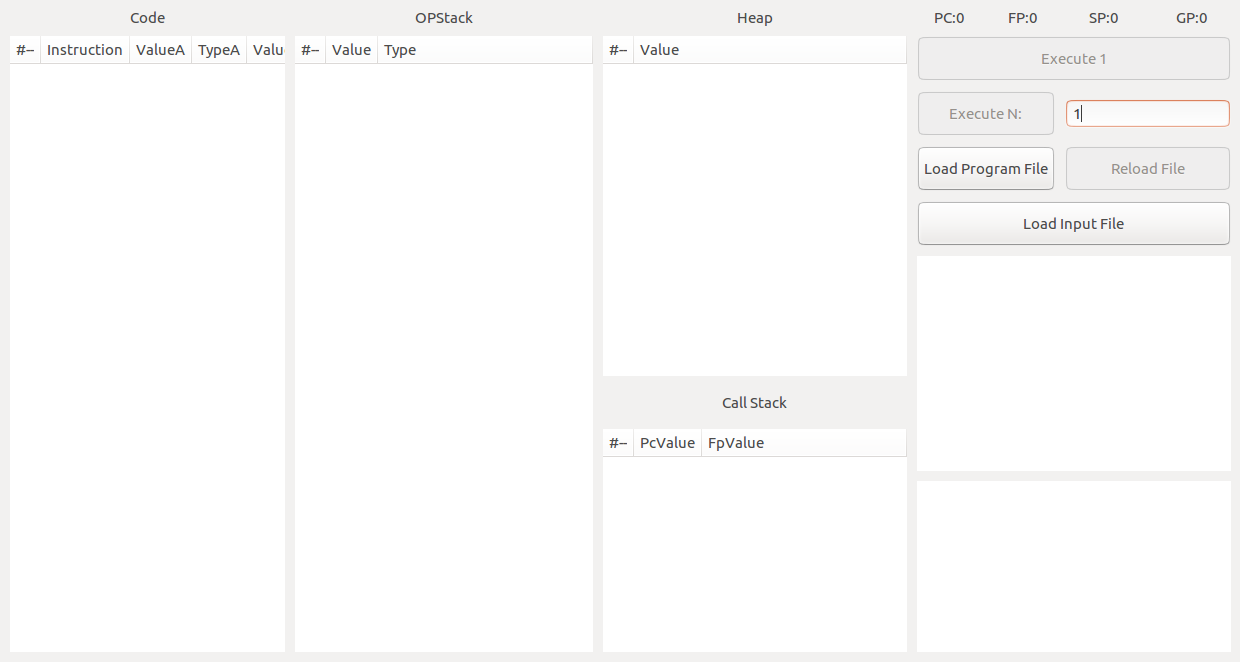
\includegraphics[width=15cm]{gtk2.png}
	\end{center}

	\begin{itemize}
		\item A informação sobre o estado das stacks encontra-se a esquerda, respetivamente
		 Code Stack / Operand Stack / Heap Stack /	Call Stack;
		\item No topo a direita e apresentada a informacao sobre todas os registos da maquina, respetivamente
			Stack Pointer / Frame Pointer /	Global Pointer /Program Counter;
		\item Execute 1 - Tal como o nome indica, executa a próxima instrução do programa;
		\item Execute N - Executa os próximos N passos, onde N e o numero que se encontra na caixa a direita; Como caso excecional,
		no caso de N ser 0, o programa será executado ate ao fim;
		\item Load Program File - Carrega um ficheiro de programa para ser executado no simulador;
		\item Reload Program File - Esta ação carrega o ficheiro na	mesma localização do ficheiro que foi carregado previamente,
		permitindo o recomeço da simulação do programa;
		\item Load Input File - Carrega um ficheiro para a zona de input (canto inferior direito);
		\item Shell - Esta janela simula a o output do modo silencioso;
		\item Janela de Input - Nesta janela e possível guardar texto para que possa ser processado como input sempre que
		o programa simulado o necessitar. Sempre que o programa necessitar de input, a primeira linha desta janela e utilizada
		a nao serque seja vazia, nesse caso e criada uma janela de input;
	\end{itemize}


\section{Mensagens de erro}

\begin{itemize}
\item \textbf{Error: Index out of array - } Provocado por um acesso indevido a zona de código, seja acesso as duas heaps ou a pilha;
\item \textbf{Error: fp == sp - } Provocado quando ...
\item \textbf{Error: Opening file - } Provocado quando ocorreu um erro a abrir um ficheiro;
\item \textbf{Error: You must specify a '-d' or '-g' option, or a program file\nTry 'man vms' for more information.\n - } Provocado quando e iniciado o simulador
com as opções/flags incorrectas;
\item \textbf{Error: Invalid type ( write / not / equal / padd second arg not int / padd first argument not adress / alocn / free /
 atox arg is not heap adress / itof / ftoi / stri / strf / loadn / load / dupn / popn / pon / storen / jz / call ) - } Provocado
 quando o(s) valores retirados da pilha/ enviados com as instruções não tem o tipo esperado;
\item \textbf{Segmentation Fault - } Provocado por um acesso indevido a zona de código, as duas heaps ou a pilha;
\item \textbf{Error \textit{mensagem} - } Provocado por uma instrução err;
\end{itemize}

\chapter{Codificação e Testes}

\section{Testes realizados e Resultados}
Durante o desenvolvimento do teste foram realizados vários programas para testar a correta implementação, mostram-se
a seguir alguns testes feitos e os respetivos resultados obtidos:\\







\noindent
\par
\begin{Parallel}[v]{0.48\textwidth}{0.48\textwidth}

\quad Teste 3x9=? (3vezes9.vm):
\ParallelLText{\noindent
	\null\begin{verbatim}
	start
			pushi 3
			pushi 9
			mul
			pushs "3 vezes 9 = "
			writes
			writei
			pushs " \n"
			writes
stop
	\end{verbatim}
}
\ParallelRText{\noindent
\quad Resultado:\\
		\begin{verbatim}
			> vms 3vezes9.vm
		3 vezes 9 = 27
		\end{verbatim}
}
\ParallelPar
\end{Parallel}

\null\\
Teste Maior de 2 Números (maior2numLidos.vm):

\noindent
\par
\begin{Parallel}[v]{0.48\textwidth}{0.48\textwidth}

\ParallelLText{\noindent
	\null\begin{verbatim}
	start
	pushi 0
	pushi 0

	pushs "introduza um numero inteiro:"
	writes
	read
	atoi
	storeg 0
	pushs "introduza um numero inteiro:"
	writes
	read
	atoi
	storeg 1
	pushg 1

	\end{verbatim}
}
\ParallelRText{\noindent
		\begin{verbatim}
			pushg 0
			supeq
			jz amaior
			pushs "O maior e: "
			writes
			pushg 1
			writei
			jump fim
			amaipushs "O maior e: "
		  writes
			pushg 0
			writei
			fim: stop
		\end{verbatim}
}
\ParallelPar
\end{Parallel}






\noindent
\par
\begin{Parallel}[v]{0.48\textwidth}{0.48\textwidth}
\null\\
\quad Testes:
\ParallelLText{\noindent
	\null\begin{verbatim}
	 > vms 5-maior2numLidos.vm
introduza um numero inteiro:49129
introduza um numero inteiro:3556
O maior e: 49129⏎
	\end{verbatim}
}
\ParallelRText{\noindent
\quad
		\begin{verbatim}
		>	 vms 5-maior2numLidos.vm
introduza um numero inteiro:-12
introduza um numero inteiro:14
O maior e: 14⏎
		\end{verbatim}
}
\ParallelPar
\end{Parallel}
\null\\\null\\
\quad Calculadora de Factorial (factorial.vm):

\noindent
\par
\begin{Parallel}[v]{0.48\textwidth}{0.48\textwidth}

\ParallelLText{\noindent
	\null\begin{verbatim}
	pushi 0
	pushi 0
	pushi 0
start
	pushi 1
	storeg 2
	pushs "enter a number\n"
	writes
	read
	atoi
	storeg 1
	pushi 1
	storeg 0
inif1: nop
	pushg 0
	pushg 1
	infeq
	jz endf1
	jump instrf1
ultinstrf1: nop
	\end{verbatim}
}
\ParallelRText{\noindent
		\begin{verbatim}
			pushg 0
			pushi 1
			add
			storeg 0
			jump inif1
		instrf1: nop
			pushg 2
			pushg 0
			mul
			storeg 2
			jump ultinstrf1
		endf1: nop
			pushs "factorial of "
			writes  //escrever
			pushg 1
			writei  //escrever
			pushs " = "
			writes   //escrever
			pushg 2
			writei  //escrever
		stop
		\end{verbatim}
}
\ParallelPar
\end{Parallel}


Testes:

\noindent
\par
\begin{Parallel}[v]{0.48\textwidth}{0.48\textwidth}

\ParallelLText{\noindent
	\null\begin{verbatim}
	> vms factorial.vm
enter a number to calculate it's factorial
7
factorial of 7 = 5040⏎
	\end{verbatim}
}
\ParallelRText{\noindent
		\begin{verbatim}
			> vms factorial.vm
			enter a number to calculate it's factorial
			10
			factorial of 10 = 3628800⏎
		\end{verbatim}
}
\ParallelPar
\end{Parallel}

















\chapter{Conclusão} \label{concl}
\quad Neste relatório descreveu-se o processo de conceção e implementação do trabalho no
âmbito da Unidade Curricular de Projecto, do curso de Licenciatura em Ciências da Computação, Universidade do Minho, no
segundo semestre do ano letivo 2017/2018. pedido pelo
enunciado, nomeadamente o parser, o simulador e a interface gráfica, alem de descrever em detalhe
o funcionamento da maquina referida.\\\\
\null\quad Os requisitos impostos pelo enunciado a que este relatório é referente são cumpridos pelos programas desenvolvidos,
os quais são apresentados neste relatório. Foram também implementadas várias funcionalidades adicionais.\\
\null\quad Apesar de estarmos satisfeitos com o trabalho desenvolvido, há ainda espaço para muitas
melhorias desta implementação. Enumeram-se algumas ideias que, por falta de tempo, não foram
(ainda) concretizadas:

\begin{itemize}
\item Criar um conjunto grande de ficheiros de testes, que sirvam tanto para provar/verificar a
implementação da maquina, assim como servir de exemplo da correta instalação da mesma;
\item Fazer melhorias no espaçamento da interface gráfica, permitindo a utilização mais fácil em janelas mais pequenas;
\item Para fins de comparação, achamos importante que no final da execução seja apresentado no modo de execução de debug
 de forma elegante o estado final das stacks, o que não acontece;
\end{itemize}

%\bibliographystyle{alpha}
%\bibliography{relprojLayout}

\end{document}
